\documentclass{article}
%----------------------------------------------------------------------------------------
%	PACKAGES AND OTHER DOCUMENT CONFIGURATIONS
\usepackage[utf8]{inputenc}
\usepackage{graphicx}
\usepackage{tabularx}
\usepackage[export]{adjustbox}
\usepackage{paralist}
\usepackage{wrapfig}
\usepackage{geometry}
 \geometry{
 a4paper,
 total={170mm,257mm},
 left=20mm,
 top=20mm,
 }

%----------------------------------------------------------------------------------------
\newcommand*{\plogo}{\fbox{$\mathcal{PL}$}} % Generic publisher logo

%----------------------------------------------------------------------------------------
%	TITLE PAGE
%----------------------------------------------------------------------------------------

\newcommand*{\titleGP}{\begingroup % Create the command for including the title page in the document
\centering % Center all text
\vspace*{\baselineskip} % White space at the top of the page

\rule{\textwidth}{1.6pt}\vspace*{-\baselineskip}\vspace*{2pt} % Thick horizontal line
\rule{\textwidth}{0.4pt}\\[\baselineskip] % Thin horizontal line

{\LARGE Caracal Automated Marking \\ Software Requirements \\ Specification}\\[0.2\baselineskip]  % Title 

Version: (1.0.0) 


\rule{\textwidth}{0.4pt}\vspace*{-\baselineskip}\vspace{3.2pt} % Thin horizontal line
\rule{\textwidth}{1.6pt}\\[\baselineskip] % Thick horizontal line

\scshape % Small caps
\vspace*{2\baselineskip} % Whitespace between location/year and editors

Edited by \\[\baselineskip]
{\Large Oratile Motswagosele \\ Mankgwanyane Tlaka \\ Lesego Makaleng \\ Kenneth Mangwane \\ Tlou Lebelo\par} % Editor list

{\itshape University of Pretoria\par} % Editor affiliation

\begin{figure}[t]
\centering
	
\includegraphics[width=350px]{UP_Logo.PNG}
\end{figure}

{\scshape 2017} \\[0.3\baselineskip] % Year published
{ Project Client: Caracal Research}\par % Publisher

\endgroup}

%----------------------------------------------------------------------------------------
%	BLANK DOCUMENT
%----------------------------------------------------------------------------------------

\begin{document} 

\titleGP % This command includes the title page
\pagebreak

\clearpage
\tableofcontents
\clearpage

\section{Introduction}

E-learning is a topic that is receiving a huge amount of attention worldwide and especially in South Africa. Currently most e-learning in schools consists of taking paper material and making it available on electronic devices such as tablets. \\ 

LMS systems such as Moodle gives the option to design and enter electronic courses and presenting assessments in the form of multiple choice and other one-dimensional methods. The available commerical systems are available but cost is a problem.

\section{Vision}

Caracal Automated Marking is aimed at  developing a metalanguage for the electronic assessment of grade 12 mathematical question in which the steps employed to arrive at the answer can be assessed, not only the final answer. The system should be ideally available as a Moodle plugin. \\

The proposed solution, ideally would be integrated into the Moodle open learning platform as a plugin. The system should accept three documents- i.e., a document with mathematics question; a document with the memorandum and a document with student answers. The system should analyze answer document and give a mark. \\

At the end the proposed  system should ideallly act as methodology through which any given problem and matching memorandum can be entered. 

\section{Background}

E-learning is a topic that receives a lot of attention worldwide and even more in Africa. The problem of educating dispersed people with few resources is a headache that troubles many government and new initiatives are being launched daily to try and solve the problem. \\

Taking a deeper look at the grade 12 question paper marking process, it is realised that most of the time, individuals are still needed who have the knowledge and skill to go through all the answered mathematics scripys and grade them correctly. This process has proven to be time costly and human error tends to creep up at a minimal level.

\section{Architecture requirements}

	\subsection{Access channel requirements}
	%place text here
	
The Caracal Automated Marking system will be web-based, and available as a Moodle plugin. Therefore it should be accessible on most platforms such as Android, Unix and iOS. Also, the browser support may be dependent on the implemented system plug-ins, however, currently Moodle 2.8 browser support is as follows:
	\begin{itemize}
		\item Google Chrome (Min. Version: 30.0 and Rec. Version: Latest)
		\item Mozilla Firefox (Min. Version: 25.0 and Rec. Version: Latest)
		\item Apple Safari (Min. Version 6 and Rec. Version: Latest)
		\item Microsoft Internet Explorer (Min. Version 9 and Rec. Version: Latest)
	\end{itemize}
Also, Moodle provides accessibility plug-ins. With the requirements listed above, the system should therefore be accessible.
	\subsection{Quality requirements}	
	%place text here
	\subsection{Integration requirements}
	%External Technologies and Software that we will be using to implement solution
	\begin{enumerate}
		\item Data Management
		\begin{itemize}
			\item Apache Flink - This is a data streaming platform that will be used to manage the streaming of data such as memo and test documents, user registrations and marking requests.
		\end{itemize}
		\item Optical Character Recognition (OCR)
		\begin{itemize}
			\item Mathpix - This is an API used to read handwritten mathematical equations, graphs, matrices etc. It will be used to read math equations from the memos and test papers of the users.
			\item AbbyyOCR4 CLI Linux - This is another API which also reads handwritten characters from scanned documents and images. This API will be used to read all characters, especially for math questions such as sequence and series and also financial math questions for compound interest, simple interest etc.
		\end{itemize}
	\end{enumerate}
	\subsection{Architecture constraints}	
	%Any constraints the client may have specified in terms of the solution space of this project
	\begin{itemize}
		\item A web based solution. This means we need to use web-technologies such as php, html in our solution, esspecially for the user interface.
		\item Moodle programming. The solution should be rendered as a moodle plugin (ideally).
	\end{itemize}
\section{Functional requirements and application design}

	\subsection{Modularization}
		\begin{enumerate}
			\item \textbf{Access Module} \\
							\textit{Scope:}\\
							 The scope of this module will be to give users a graphical user interface, which will allow them to login and register and to also be able to have access to the system as the whole. This module will be in charge of deploying a GUI on multiple browsers i.e. FireFox, Google Chrome, Microsoft Edge. It will provide a friendly user functionality of the whole system.  
\begin{itemize}
						\item use case diagrams\\
								\begin{figure}[h]
								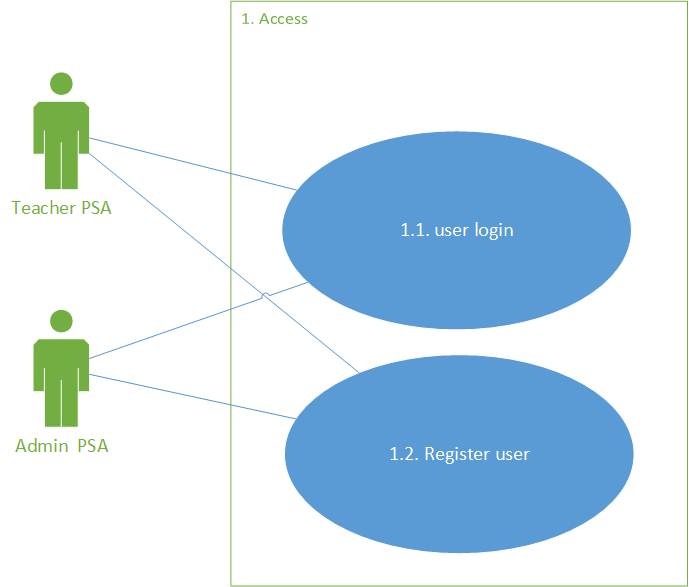
\includegraphics[width=200px, height=200px]{access.png}
								\caption{I/O module use case diagram}
								\end{figure}
\end{itemize}
			\item \textbf{User Management Module}\\
						\textit{Scope:}\\
						This module will be in charge of managing user information and the different types of users. The different types of users of this system will be as follows: \\
						\begin{itemize}
							\item Admin - The role of this user will be to have access to uploading question papers and memorandums, and general access to sensitive information of the system. This user can also delete/approve other users below this level i.e. Teachers from the system. 
							\item Teacher - The role of this user will be to upload the test papers of students i.e. their class of students, and recieve marks of the papers they have uploaded. This user cannot have direct access to the memo or question paper. This user also needs approval from the admin before being registered. This is to prevent students registering as fake teachers and uploading tests to get access to the marking system 
						\end{itemize}
\begin{itemize}
								\item use case diagrams\\
								\begin{figure}[h]
								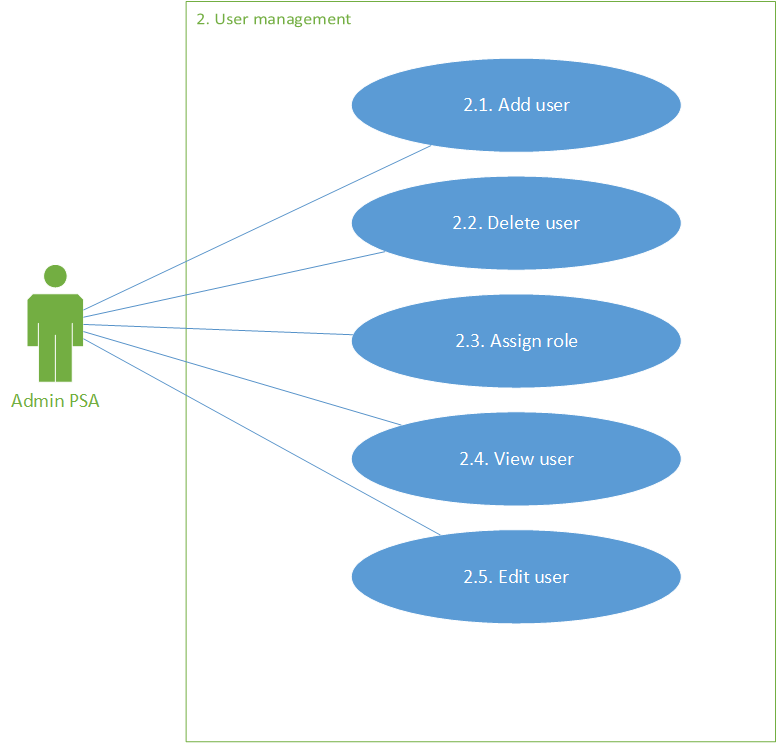
\includegraphics[width=200px, height=200px]{user_management.png}
								\caption{user management module use case diagram}
								\end{figure}
						\end{itemize}
			\item \textbf{Notifications Module}\\
						\textit{Scope:}\\
						This module will be responsible for giving feedback to the users of the system. A general example would be when a teacher uploads 100 papers to be marked. If the system can't handle the request immediately, the notifications module will have to notify that teacher when their papers are ready to be retrieved after marking is completed. The module will deploy notifications via notices on the system and also emails for more complex notifications like paper collection.
					\begin{itemize}
								\item use case diagrams\\
								\begin{figure}[h]
								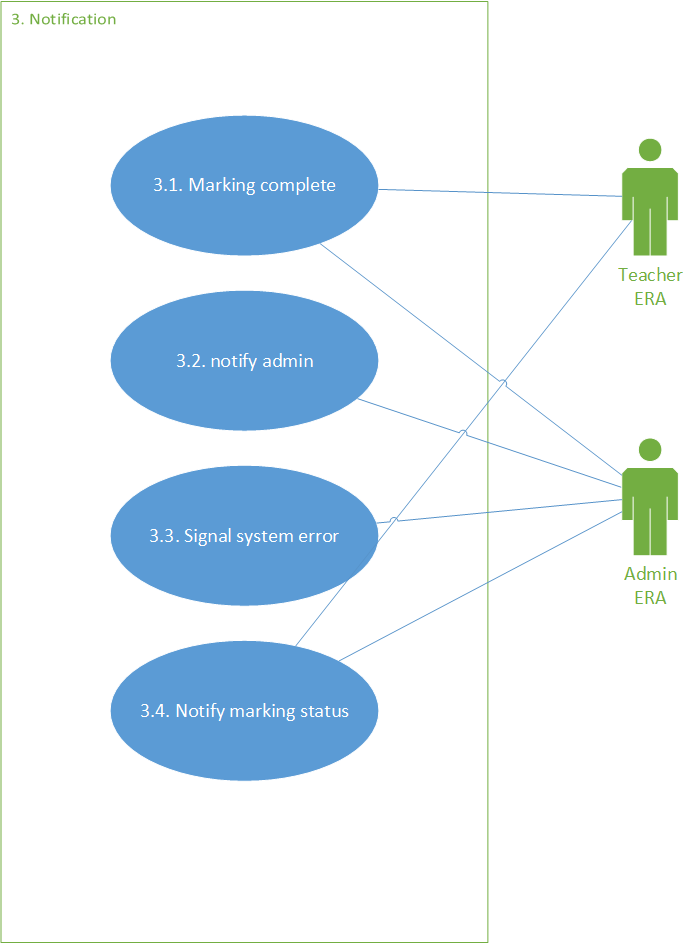
\includegraphics[width=200px, height=200px]{notification.png}
								\caption{Notifications module use case diagram}
								\end{figure}
						\end{itemize}

			\item \textbf {Data Streaming and Security Module}\\
					\textit{Scope:}\\
					This module will be responsible for handling and management of data in all its forms. The module will firstly make sure that requests relating to data uploads and downloads are handled as quick as possible through an external data management tool API. The module will also make sure that before data is transported from server to client and vica versa, it will be decrypted and encrypted respectively. This module will basically be responsible for data integrity and data protection of the system.  \\
			\begin{itemize}
								\item use case diagrams\\
								\begin{figure}[h]
								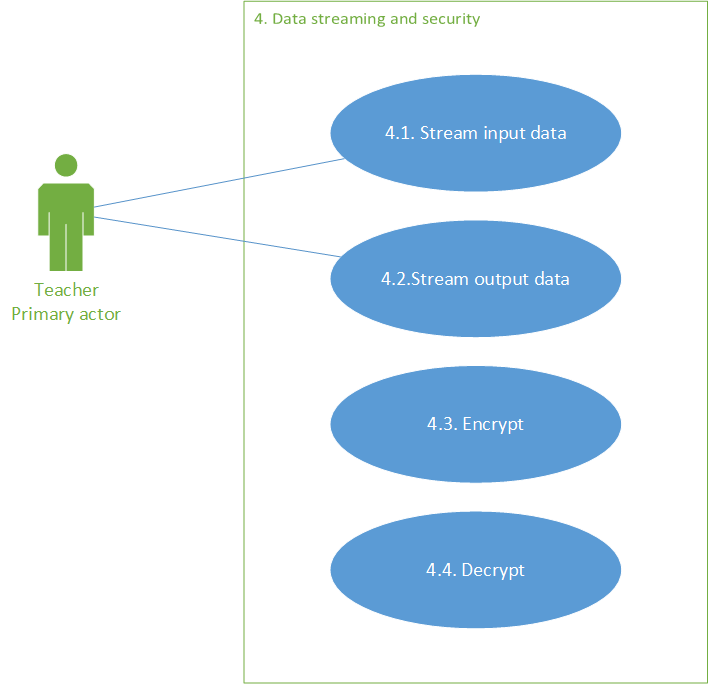
\includegraphics[width=200px, height=200px, inner]{data_and_security.png}
								\caption{data and security module use case diagram}
								\end{figure}
					\end{itemize}
			
			\item \textbf{Marking Module}\\
				\textit{Scope:}\\
				This module will be responsible for the actual marking of uploaded scripts. This module will perform at least 3 functions, which are:
				\begin{itemize}
					\item Paper Slicing - This means that the paper will be analyzed, and broken into smaller pieces for OCR functionality.
					\item Comparing - This means after breaking the paper in smaller pieces, AI analytical algorithms will be used to properly compare and mark the answers against the memo.
					\item Persisting - This means after marking is complete, the marks and relevant answer sheet will be stored in the database.
				\end{itemize}
\begin{itemize}
								\item use case diagrams\\
								\begin{figure}[h]
								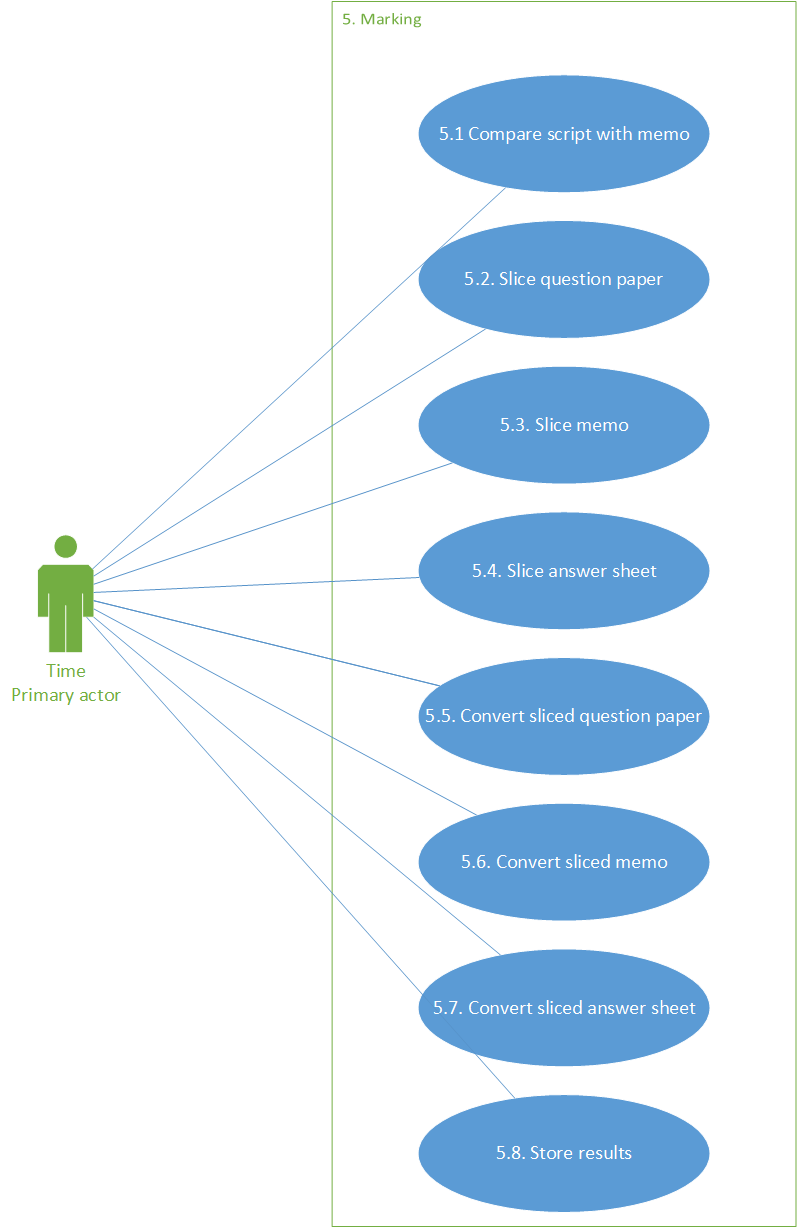
\includegraphics[width=200px, height=200px]{marking.png}
								\caption{marking module use case diagram}
								\end{figure}
					\end{itemize}
			\item \textbf{Reporting Module}\\
			
				\textit{Scope:}\\
				The Scope of this module will be to create performance and statistical reports of the student marks and basically give feedback of how the marks went, what problems most students faced, suggestions etc. This module will compile a report using data from the database and analytical data algorithms. 
			\begin{itemize}
								\item use case diagrams\\
								\begin{figure}[h]
								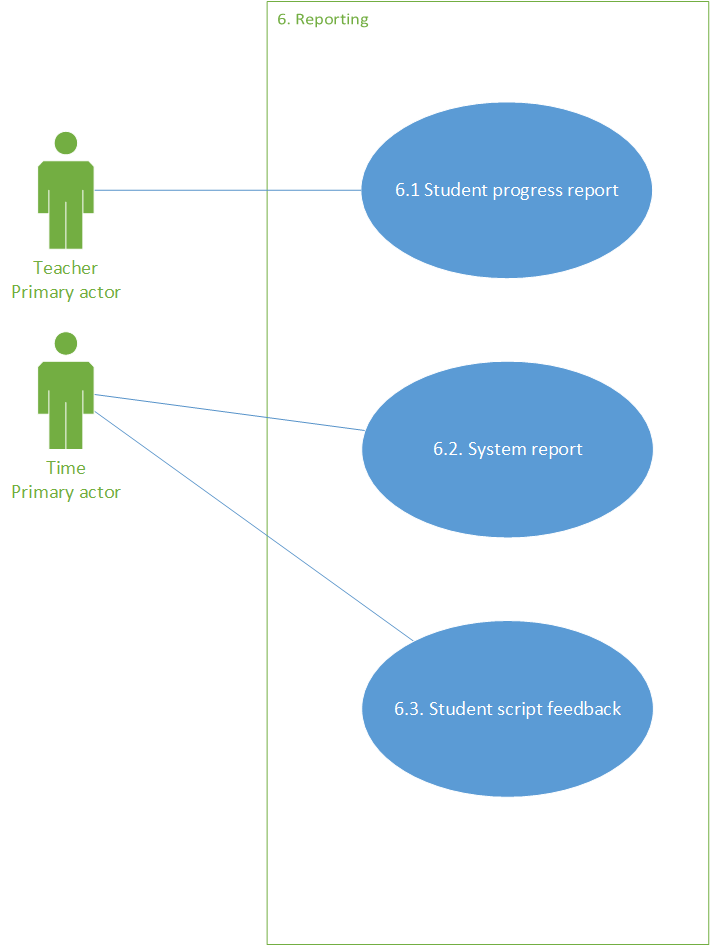
\includegraphics[width=200px, height=200px]{reporting.png}
								\caption{reporting module use case diagram}
								\end{figure}
					\end{itemize}
			\item \textbf{I/O Module}\\
		
				\textit{Scope:}\\
				This module will be in charge of the inputting and outputting of documents. One of the core functionalities for this module, will be to edit the answer sheet and append the marks calculated by the marking module to the answer sheet, and then outputting that document back to the user for download. Managing where documents are inputted to, formats and structure will also be amongst the scope of this module.
			\begin{itemize}
								\item use case diagrams\\
								\begin{figure}[h]
								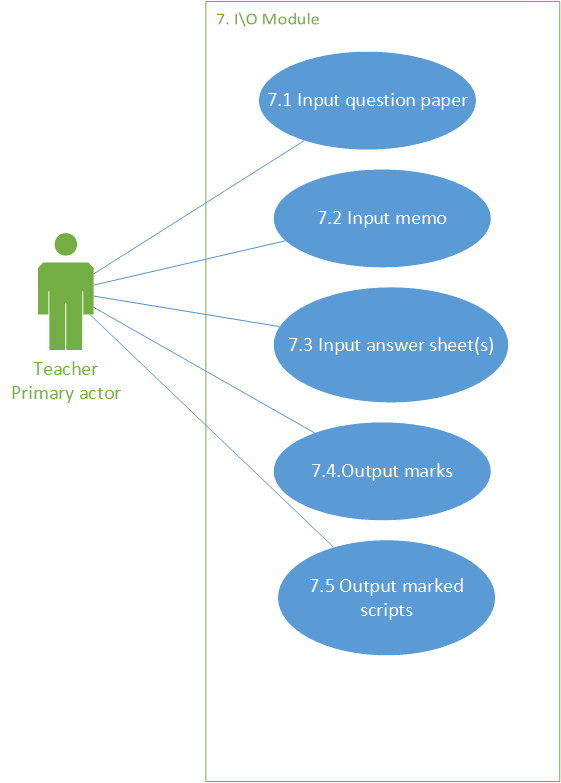
\includegraphics[width=200px, height=200px]{io_module.png}
								\caption{I/O module use case diagram}
								\end{figure}
					\end{itemize}
			
		\end{enumerate}
	\subsection{Use case prioritization}

		\subsubsection{Critical:}
			\begin{itemize}
				\item Register User
				\item Input Question Paper
				\item Input Memo
				\item Input Student Answer Script
				\item Save All Input Files
				\item Compare Student Answer Script against Memo
				\item Persist and save obtained mark
				\item Output Marks
				\item Output Marked Script
			\end{itemize}
		\subsubsection{Important:}
			\begin{itemize}
				\item Validate User Information/Credentials
				\item Validate Question Paper
				\item Validate Memo
				\item Validate Student Answer Script
				\item Slice Question Paper
				\item Slice Memo
				\item Slice Student Answer Script
				\item Convert Sliced Question Paper Sections To Suitable Format
				\item Convert Sliced Memo Sections To Suitable Format
				\item Convert Sliced Student Answer Script Sections To Suitable Format
				\item Associate Sliced Question Paper Section; Memo Section And Student Answer Script Section with Student Details
				
			\end{itemize}
		\subsubsection{Nice-To-Have:}
			\begin{itemize}
				\item Find Student Details From Answer Script
				\item Compile a report which includes information such as highest marks, average, lowest, overall performance etc.
				\item Learn Way Of Answering
				\item Reason For Given Mark
			
			\end{itemize}
	\subsection{Use case/Services contracts}
\subsection{Critical:}

\begin{itemize}
	
		\item Input memo
			\begin{itemize}
				\item Pre-condition \\
					 The must be a memo and a scannig system that can accept the memo in physcical form. If the memo is already in the required format which is pdf, the system will accept the input in the pdf format.
				\item Post-condition \\
					 The output will be a bmp image and a pdf document.
			\end{itemize}
		\item Input  question paper
			\begin{itemize}
				\item Pre-condition \\
					 The must be a question paper and a scannig system that can accept the question paper in physcical form. If the question paper is already in the required format which is pdf, the system will accept the input in the pdf format.
				\item Post-condition \\
					 The output will be a bmp image and a pdf document.
			\end{itemize}
		\item Input  student answer script
			\begin{itemize}
				\item Pre-condition \\
					 The must be an answer script and a scannig system that can accept the answer script in physcical form. 
				\item Post-condition \\
					 The output will be a bmp image and a pdf document.
			\end{itemize}


		\item Mark script
			\begin{itemize}
				\item Pre-condition \\
					 The answer script must be available in the system as a bmp image and/or a pdf document(and the input files must have passed analysis).
				\item Post-condition \\
					 The marks obtained by the student
			\end{itemize}
			
		\item Persist Obtained mark
			\begin{itemize}
				\item Pre-condition \\
					 The system should be done marking with no errors.
				\item Post-condition \\
					 The marks are matched with the student in put in the database.
			\end{itemize}

		\item Output marks
			\begin{itemize}
				\item Pre-condition \\
					 The marks must be available in the database
				\item Post-condition \\
					 The system shows the marks of the required student.
			\end{itemize}
		\item Output marked sheet
			\begin{itemize}
				\item Pre-condition \\
					 The system should be done marking with no errors.
				\item Post-condition \\
					 The system prints out the marked answer sheet
			\end{itemize}

			


\end{itemize} 

\subsubsection{Important:}
	\begin{itemize}
		\item Validate Question Paper
			\begin{itemize}
				\item Pre-condition \\
					 The must be a question paper saved in the system as a bmp image or pdf document.
				\item Post-condition \\
					 An error if the question paper is not readable or corrupted.
			\end{itemize}
		\item validate Memo
			\begin{itemize}
				\item Pre-condition \\
					 The must be a memo saved in the system as a bmp image or pdf document.
				\item Post-condition \\
					 An error if the memo is not readable or corrupted.
			\end{itemize}
		\item validate Student Answer Script
			\begin{itemize}
				\item Pre-condition \\
					 The must be a answer sheet saved in the system as a bmp image or pdf document.
				\item Post-condition \\
					 An error if the answer sheet is not readable or corrupted.
			\end{itemize}
		\item Slice Question Paper
			\begin{itemize}
				\item Pre-condition  \\
					 The must be a question paper saved in the system as a bmp image or pdf document.
				\item Post-condition \\
					 The question paper will be split into small subsections and stored in a temporary database in the system
			\end{itemize}
		\item Slice Memo
			\begin{itemize}
				\item Pre-condition  \\
					 The must be a memo  saved in the system as a bmp image or pdf document.
				\item Post-condition \\
					 The question paper will be split into small subsections and stored in a temporary database in the system
			\end{itemize}
		\item Slice Student Answer Script
			\begin{itemize}
				\item Pre-condition  \\
					 The must be an answer sheet saved in the system as a bmp image or pdf document.
				\item Post-condition \\
					 The answer sheet will be split into small subsections and stored in a temporary database in the system
			\end{itemize}
		\item Convert Sliced  Question Paper Sections To Suitable Format
			\begin{itemize}
				\item Pre-condition \\
					 The must be a question paper in  the system that has been sliced into small subsections
				\item Post-condition \\
					 The question paper subsections will be converted to a format suitable to the format accepted by the marking system
			\end{itemize}
		\item Convert Sliced  Memo Sections To Suitable Format
			\begin{itemize}
				\item Pre-condition \\
					 The must be a memo in  the system that has been sliced into small subsections
				\item Post-condition \\
					 The memo subsections will be converted to a format suitable to the format accepted by the marking system
			\end{itemize}
		\item Convert Sliced  Student Answer Script Sections  To Suitable Format
			\begin{itemize}
				\item Pre-condition \\
					 The must be a answer sheet in  the system that has been sliced into small subsections
				\item Post-condition \\
					 The answer sheet subsections will be converted to a format suitable to the format accepted by the marking system
			
			\end{itemize}


	\end{itemize}

		\subsubsection{Request and Results Data Structures:}
		%place text here
	\subsection{Required functionality}
	%place text here
	
The Caracal Automated Marking system will mostly rely on the the Optical Character Recognition (OCR), which has three most essential elements that are vital for the Caracal Automated Marking system. The elements are scanning, reading text and recognition. Therefore, as shown in Figure 1 below, the sequential or rather logical flow of the system will be input, scanning conversion, marking and output.

\begin{figure}[t]
	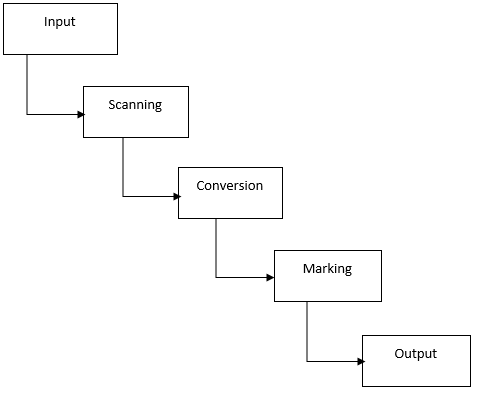
\includegraphics[width=\linewidth]{flow.PNG}
	\caption{Caracal Automated Marking logical flow}
\end{figure}


The system accept documents as input, with the integrated OCR technology the input documents have to be scanned and stored temporarily as images for marking. The images are then converted into words and characters that are recognizable. Next, the system marks the document, stores the marks and produce the output. The output is preferably the marked document as a portable document file. Therefore the overall functionality of the Caracal Automated Marking will be:
	\begin{itemize}
		\item Input - Three documents (i.e Question paper, Memo and the Answer sheet)
		\item Validation and Scanning
		\item Conversion
		\item Marking
		\item Output - Marked document as portable document file
	\end{itemize}
	\subsection{Process specification}
	\begin{figure}[h]
	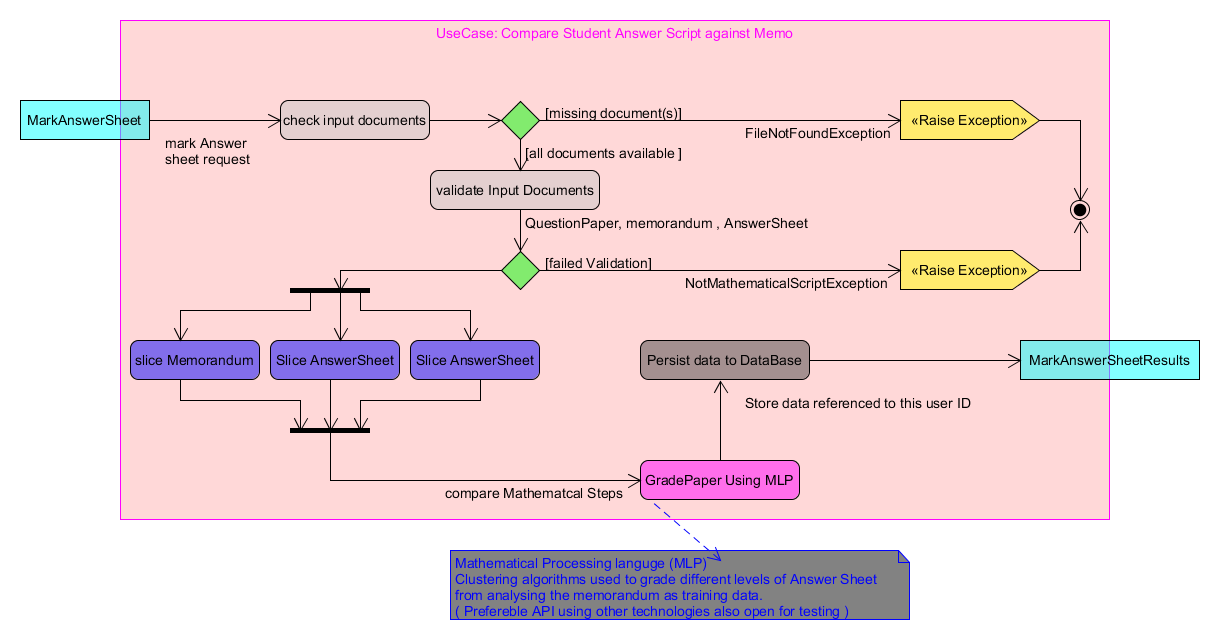
\includegraphics[width=\linewidth]{processSpecification.png}
	\caption{Caracal Automated Marking Process Specification Diagram}
	\end{figure}
	\subsection{Domain Model}
	\begin{figure}[h]
		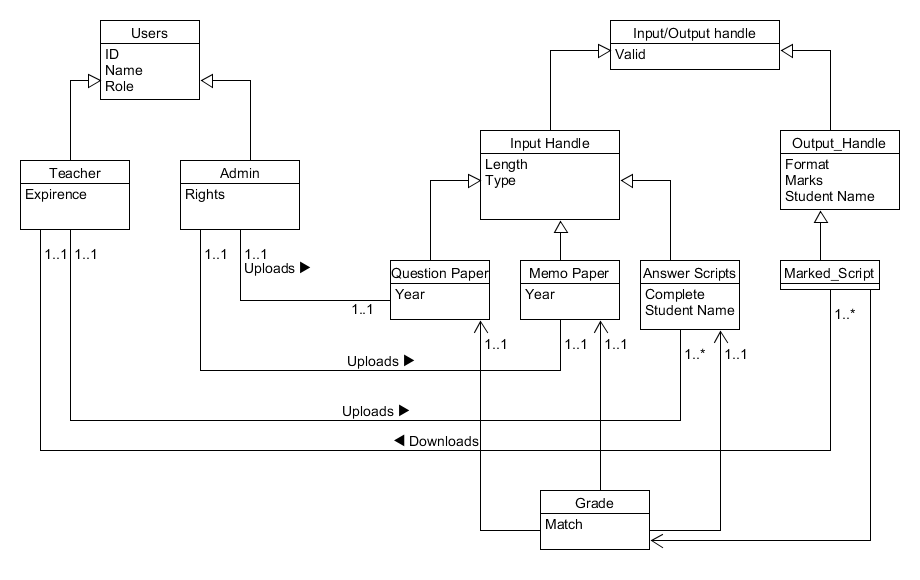
\includegraphics[width=\linewidth,height=245px]{Domain_Model.png}
		\caption{Caracal Automated Marking Domain Model}
	\end{figure}
    \subsection{Traceability Matrix}
	\subsubsection{Use Cases}
	\begin{itemize}
	\item UC1.1: User Login
	\item UC1.2: Register User
	\item UC2.1: Add User
	\item UC2.2: Delete User
	\item UC2.3: Assign Role
	\item UC2.4: View User
	\item UC2.5: Edit User
	\item UC3.1: Notify Marking Status
	\item UC3.2: Notify Admin
	\item UC3.3: Signal System Error
	\item UC4.1: Stream Input Data
	\item UC4.2: Stream Output Data
	\item UC4.3: Encrypt
	\item UC4.4: Decrypt
	\item UC5.1: Compare Script with Memo
	\item UC5.2: Slice Question Paper
	\item UC5.3: Slice Memo
	\item UC5.4: Slice Answer Sheet
	\item UC5.5: Convert Sliced Question Paper
	\item UC5.6: Convert Sliced Memo
	\item UC5.7: Convert Sliced Answer Sheet
	\item UC5.8: Store Results
	\item UC6.1: Produce Student Performance Report
	\item UC6.2: Produce System Report
	\item UC6.3: Student Script Feedback
	\item UC7.1: Input Question Paper
	\item UC7.2: Input Memo
	\item UC7.3: Input Answer Sheet(s)
	\item UC7.4: Output Marks
	\item UC7.5: Output Marked Script
	\end{itemize}
	\subsection{Requirements}
	\begin{itemize}
	\item R01: Present Usable and Responsive Interface
	\item R02: Enable Login Functionality for Users
	\item R03: Allow New Users to Register
	\item R04: Allow for Document Input
	\item R05: Answer Sheet Marking
	\item R06: Notifications
	\item R07: Output: Marked Answer Sheet
	\end{itemize}
\begin{table}[h!]
\centering
\label{my-label}
\begin{tabular}{|l|l|l|l|l|l|l|l|l|l|l|l|l|l|}
\hline
Requirement & Priority & \begin{tabular}[c]{@{}l@{}}UC\\ 1.1\end{tabular} & \begin{tabular}[c]{@{}l@{}}UC\\ 1.2\end{tabular} & \begin{tabular}[c]{@{}l@{}}UC\\ 2.1\end{tabular} & \begin{tabular}[c]{@{}l@{}}UC\\ 3.1\end{tabular} & \begin{tabular}[c]{@{}l@{}}UC\\ 5.1\end{tabular} & \begin{tabular}[c]{@{}l@{}}UC\\ 5.8\end{tabular} & \begin{tabular}[c]{@{}l@{}}UC\\ 7.1\end{tabular} & \begin{tabular}[c]{@{}l@{}}UC\\ 7.2\end{tabular} & \begin{tabular}[c]{@{}l@{}}UC\\ 7.3\end{tabular} & \begin{tabular}[c]{@{}l@{}}UC\\ 7.4\end{tabular} & \begin{tabular}[c]{@{}l@{}}UC\\ 7.5\end{tabular} \\ \hline
R01 & 1 & X & X &   &    &    &    &    &    &    &    &    \\ \hline
R02 & 2 & X &   & X &    &    &    & X  & X  & X  &    &    \\ \hline
R03 & 2 & X & X & X &    &    &    &    &    &    &    &    \\ \hline
R04 & 1 &   &   &   &    & X  &    & X  & X  & X  &    &    \\ \hline
R05 & 1 &   &   &   &    & X  & X  &    &    &    & X  & X  \\ \hline
R06 & 3 &   &   &   & X  &    &    &    &    &    &    &    \\ \hline
R07 & 2 &   &   &   &    &    & X  &    &    &    & X  & X   \\ \hline
\multicolumn{2}{|c|}{UC Priority} & 1 & 2 & 2 & 1 & 2 & 1 & 1 & 1 & 1 & 1 & 2   \\ \hline
\end{tabular}
\caption{Traceability Matrix}
\end{table}

\section{Open Issues}
	 The most critical issue is if the client is willing to pay for the technologies that we are going to use or should we develop everything from scratch. Another issue is the format of the question paper and memo, how is the question paper and memo going to be structured and is the structure going to be conbsistent or should our system adapt to any structure that it is presented. Will the system mark the final answer or should it also mark the steps followed to get the answer. \par
	 Should the system write the marks on the answer sheet or should it print a copy with the marks of the student. Will the scripts be entered one at the time then marked or will the system accept a load of scripts and then mark every sheet. 

\end{document}
